\section{Einleitung in die Thesis} \label{Einleitung in die Thesis}

Das Institut für Intelligente Industrielle Systeme (I3S) befasste sich im Rahmen von Forschungsprojekten bereits mit der Thematik von skill-basierten Softwareansätzen. ROS war dabei ein zentrales Element der Entwicklung. Jedoch gab es weiterhin viele offene Fragen in Bezug auf den Einsatz von Skills. 
\\
Die Thesis wird mit der Idee initialisiert, neue Ansätze und Herangehensweisen zu finden und zu erarbeiten. Der Fokus liegt auf einer industrienahen Umsetzung und den Einsatz einer SPS. Bereits gewonnene Erfahrungen aus Projekten im Bereich der Verfahrenstechnik sollen in die Entwicklung neuer Ansätze einfliessen. Dabei wird die Frage erarbeitet, welche Parallelen es zur Verführungstechnik gibt und wie diese für Skill-Anwendungen übernommen werden könnten. 
 
\vspace{2mm} 
Die Thesis setzt sich mit grundlegenden Fragen auseinander, wie:
\begin{itemize}
	\item Was ist ein Skill und für welche Aufgaben eignet sich der Einsatz dieser.
	\item Wie kann ein Skill definiert werden.
	\item In welche Software-Struktur muss ein Skill eingebettet werden. 
	\item Welche Möglichkeiten und Grenzen hat der Einsatz von Skills.
\end{itemize}
\vspace{3mm} 

Das allgemeine Vorgehen innerhalb des Projektes folgt dabei den klassischen Entwicklungs-Phasen (Analyse / Konzipieren / Ausarbeitung / Auswertung). Zu Beginn wird eine ausführliche Analyse der Thematik, durchgeführt um alle themenrelevanten Fragen zu beantworten. Anhand dieser Analyse werden die diversen Arbeitspakete des Projektes definiert, welche jeweils mit einer Konzept- und Ausarbeitungsphase umgesetzt werden. Die Dokumentation dieser Thesis konzentriert sich darauf, den Entwicklungsprozess sowie die zugrunde liegenden Überlegungen detailliert darzustellen. Der Fokus liegt dabei auf der Beschreibung der methodischen Herangehensweise und der Schritte, die zur Erarbeitung der finalen Lösung geführt haben. Ziel ist es, transparent nachzuvollziehen, wie die Lösung entwickelt wurde und welche Entscheidungen den Prozess geprägt haben.
\\
\\
Mit dem Start des Semesters am 16.09.2024 wurde auch mit der Arbeit an dieser Thesis begonnen. Die Thesis umfasst dabei ca. 900 Arbeitsstunden.  Das Projekt wird von Prof. Melchior Borer betreut und in enger Zusammenarbeit mit dem I3S umgesetzt. Dabei wird ein stetiger Austausch mit Prof. Dr. Norman Urs Baier, dem Leiter des Instituts für Intelligente Industrielle Systeme, angestrebt.  
	
\newpage
\section{Auftragsinterpretation} \label{Auftragsinterpretation}

	\textbf{Problembeschreibung:} \vspace{2mm} 
	\\
	Roboter finden in der Industrie eine immer breiter werdende Anwendung und sind aus vielen Prozessen
	nicht mehr wegzudenken. Ein grosser Beschaffungs- und Inbetriebnahmeaufwand machen es jedoch
	für viele Unternehmen schwierig, einen Roboter in ihre Prozesse zu integrieren. Dadurch werden
	zeitintensive und monotone Arbeiten oftmals noch manuell von Mitarbeitern durchgeführt. Eine grosse
	Hürde des Robotersystems ist der konventionelle Robotersoftwareansatz, welcher ein Grundverständnis
	für die Programmierung des Roboters voraussetzt. Für Veränderungen im Prozessablauf wird dadurch
	zwingend ein Programmierer benötigt.
	\vspace{3mm}
	
	\textbf{Beschreibung des Auftrages:} \vspace{2mm} 
	\\
	Die Thesis beschäftigt sich mit der Frage, wie ein Roboter einfacher und standardisiert programmiert
	werden kann. Hierfür wird der Ansatz einer Rezeptursteuerung (bekannt aus Pharmaprozessen)
	analysiert. Dabei wird untersucht, ob ein solcher Ansatz für Roboteranwendungen geeignet ist und wie
	dieser eingesetzt werden kann. Ein zentrales Element ist dabei der skill-basierte Aufbau eines
	Roboterprogramms.
	\\
	\linebreak
	Die konkreten Ziele dieser Thesis sind wie folgt definiert:
	\begin{itemize}
		\item Analyse des Ansatzes einer Rezeptursteuerung für Roboteranwendungen.
		\item Analyse und Definierung von geeigneten Skills.
		\item Softwaremässige Umsetzung des skill-basierten Ansatzes.
		\item Reaktion der Software auf Fehler des Roboters während der Prozessdurchführung.
	\end{itemize}
	\addvspace{5mm}
	
	\textbf{Auftragskontext:} \vspace{2mm} 
	\\
	Die Thesis findet als BFH-internes Projekt statt, welches aus dem Forschungsprojekt «ACROBA»
	entstanden ist. Das Ziel des ACROBA-Forschungsprojektes ist die Entwicklung und Demonstration neuartiger
	Konzepte für Roboterplattformen bezüglich agiler Fertigung.
	\vspace{3mm}
	
	\textbf{Abgrenzungen:} \vspace{2mm} 
	\\
	Die Thesis beschäftigt sich nicht mit der Umsetzung einer konkreten industriellen Anwendung. Es ist
	jedoch möglich, dass Erkenntnisse aus dieser Thesis für zukünftige Automatisierungsprojekte
	verwendet werden können.
	\vspace{3mm}
	
	\textbf{Projektorganisation:} \vspace{0mm} 
	
	\begin{table}[ht]
		\centering
		\colorlet{BFH-table}{BFH-MediumBlue!10}
		\colorlet{BFH-tablehead}{BFH-MediumBlue!50}
		\begin{bfhTabular}{llll}
			Rolle		& 	Wer							&	Status				&	Kontakt		\\\hline
			
			Advisor		 & Prof. Borer Melchior			& Dozent BFH 			& 	\href{mailto:melchior.borer@bfh.ch}{melchior.borer@bfh.ch}  	\\\hline
			Experte		 & Stucki Simon					& Externer Experte		&	/		\\\hline
			Student		 & Yannick Spatz 				& Master-Student		&	\href{mailto:yannick.spatz@bfh.ch}{yannick.spatz@bfh.ch}	\\\hline
			
		\end{bfhTabular}
		
		\captionsetup{justification=centering}
		\caption{Projektorganisation}
		\label{Projektorganisation}
	\end{table}
	

\section{Zeitplan der Thesis} \label{Zeitplan der Thesis}

	Der erstellte Zeitplan dient als erste grobe Orientierung und stellt eine vorläufige Einschätzung des Projektverlaufs dar. Da der genaue Umfang der Aufgabenstellung für diese Thesis nur schwer im Voraus vollständig abzuschätzen ist, kann der Projektrahmen entsprechend variieren. Insbesondere die Entwicklung der Software ist ein dynamischer und iterativer Prozess.
	\\
	Daher ist der Zeitplan als flexibles Arbeitstool zu verstehen, das zwar eine klare zeitliche Struktur vorgibt, sich jedoch im Laufe des Projekts an veränderte Anforderungen und Erkenntnisse anpassen kann. Er soll einerseits helfen, die einzelnen Meilensteine im Blick zu behalten und andererseits als Leitfaden dienen, um trotz aufkommender Änderungen einen festen Rahmen für den Projektfortschritt zu gewährleisten. Die kontinuierliche Überprüfung und gegebenenfalls Anpassung des Zeitplans ist ein integraler Bestandteil dieses Prozesses, um sicherzustellen, dass das Projekt im vorgesehenen zeitlichen Rahmen bleibt. 

	\begin{figure}[h!]
		\centering
		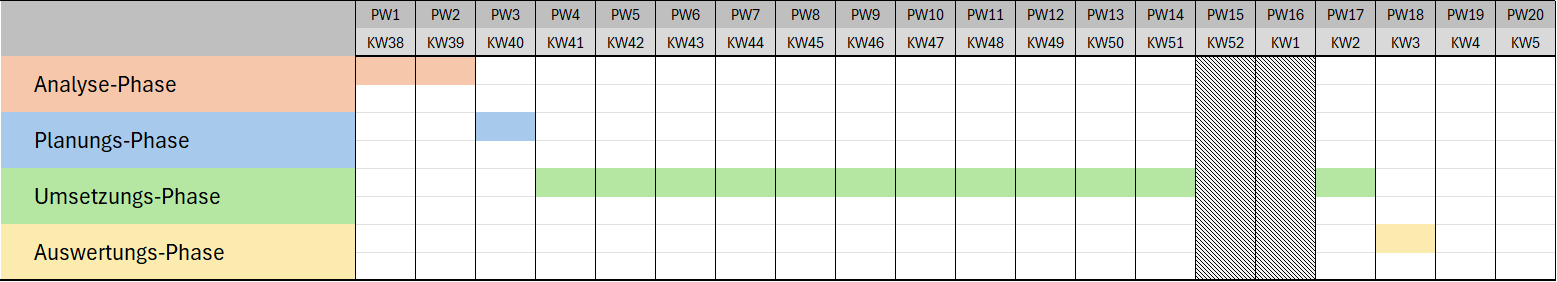
\includegraphics[width=1\textwidth]{01_Rahmen_der_Arbeit/Terminplanung_V2}
		\caption{Grobzeitplan der Thesis}
		\label{fig:Grobzeitplan}
	\end{figure}
	
	\begin{bfhNoteBox}
		Eine detaillierte Version des endgültigen Zeitplans wird im Anhang aufgeführt.
	\end{bfhNoteBox} 

		